
\section{Multiply/Divide Mixed Numbers}

In this lesson, we will learn how to multiply and divide mixed numbers. The rule is very simply: Before we multiply/divide mixed numbers, we need to change them (like $1\frac{1}{2}$) to improper fractions (like $\frac{3}{2}$), and then use fraction multiplication/division rules we learned earlier.

\subsection{Multiply/Divide Mixed Numbers}

You might need to go back to review how to change a mixed number to an improper fraction.

\begin{myexample}
\[ 
\begin{aligned}[t]
	&\phantom{{}=} 1\frac{1}{2} \cdot 3\frac{5}{6} \\
	&= \frac{3}{2} \cdot \frac{23}{6} \\
	&= \frac{3\div3}{2} \cdot \frac{23}{6\div3} \\
	&= \frac{1}{2} \cdot \frac{23}{2} \\
	&= \frac{1\cdot23}{2\cdot2} \\
	&= \frac{23}{4} \\
	&= 5\frac{3}{4}
\end{aligned}
\]
The last step is optional, depending on what the question asks. If the question doesn't ask for a mixed number answer, you could leave the answer as $\frac{23}{4}$.
\end{myexample}

\begin{myexample}
\[ 
\begin{aligned}[t]
	&\phantom{{}=} 8\frac{1}{4} \div 3 \\
	&= \frac{33}{4} \div \frac{3}{1} \\
	&= \frac{33}{4} \cdot \frac{1}{3} \\
	&= \frac{33\div3}{4} \cdot \frac{1}{3\div3} \\
	&= \frac{11}{4} \cdot \frac{1}{1} \\
	&= \frac{11}{4} \\
	&= 2\frac{3}{4}
\end{aligned}
\]
\end{myexample}

\subsection{Word Problems}

\begin{myexample}
Each truck can hold $3\frac{1}{4}$ tons of sand. In a job, it took $24$ full truck loads to transfer a certain amount of sand. How many tons of sand were transferred?
\end{myexample}
\begin{solution}
This is obviously a multiplication problem:
\[ 
\begin{aligned}[t]
	&\phantom{{}=} 3\frac{1}{4} \cdot 24 \\
	&= \frac{13}{4} \cdot \frac{24}{1} \\
	&= \frac{13}{4\div4} \cdot \frac{24\div4}{1} \\
	&= \frac{13}{1} \cdot \frac{6}{1} \\
	&= \frac{13\cdot6}{1\cdot1} \\
	&= \frac{78}{1} \\
	&= 78
\end{aligned}
\]
\textbf{Conclusion:} Those trucks transferred $78$ tons of sand.
\end{solution}


\begin{myexample}
In a running contest (with breaks), each runner will run $28$ miles. A runner runs $5\frac{1}{4}$ miles per hour. How many hours will it take the runner to complete the race?
\end{myexample}
\begin{solution}
In this problem, we need to find out how many $5\frac{1}{4}$ miles are in $28$ miles, a division problem:
\[ 
\begin{aligned}[t]
	&\phantom{{}=} 28 \div 5\frac{1}{4} \\
	&= \frac{28}{1} \div \frac{21}{4} \\
	&= \frac{28}{1} \cdot \frac{4}{21} \\
	&= \frac{28\div7}{1} \cdot \frac{4}{21\div7} \\
	&= \frac{4}{1} \cdot \frac{4}{3} \\
	&= \frac{16}{3} \\
	&= 5\frac{1}{3}
\end{aligned}
\]

\textbf{Conclusion:} It would take the runner $5\frac{1}{3}$ hours to complete the race. 

Since each hour has $60$ minutes, $\frac{1}{3}$ of an hour has $20$ minutes, so it would take the runner $5$ hours and $20$ minutes to complete the race.

In this problem, it would not be good to say it would take the runner $\frac{16}{3}$ hours to complete the race.
\end{solution}

\begin{myexample}
Find the area of the following rectangle.
\begin{center}
\begin{tikzpicture}
	\draw (0,0) rectangle (4,3);
	\draw(2,-0.5) node{$2\frac{1}{4}$ in};
	\draw(-0.5,1.5) node{$1\frac{2}{3}$ in};
\end{tikzpicture}
\captionof{figure}{Find the area of the rectangle}
\end{center}
\end{myexample}
\begin{solution}
To find the area of a rectangle, we multiply the base and the height:
\[ 
\begin{aligned}[t]
	&\phantom{{}=} 2\frac{1}{4} \cdot 1\frac{2}{3} \\
	&= \frac{9}{4} \cdot \frac{5}{3} \\
	&= \frac{9\div3}{4} \cdot \frac{5}{3\div3} \\
	&= \frac{3}{4} \cdot \frac{5}{1} \\
	&= \frac{15}{4} \\
	&= 3\frac{3}{4}
\end{aligned}
\]
\textbf{Conclusion:} The area of the rectangle is $3\frac{3}{4}$ square inches (or $\text{in}^{2}$).
\end{solution}

\begin{myexample}
Find the area of the following triangle.
\begin{center}
\begin{tikzpicture}
	\draw (0,0) -- (4,0) -- (0,3) -- (0,0);
	\draw (0,0.2) -- (0.2,0.2) -- (0.2,0);
	\draw(2,-0.5) node{$2\frac{1}{4}$ in};
	\draw(-0.5,1.5) node{$1\frac{2}{3}$ in};
\end{tikzpicture}
\captionof{figure}{Find the area of the triangle}
\end{center}
\end{myexample}
\begin{solution}

Notice that a triangle is actually half a rectangle. See the following figure:
\begin{center}
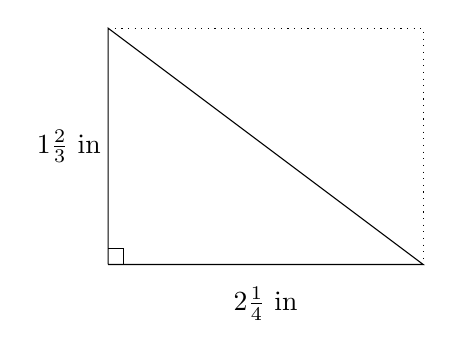
\begin{tikzpicture}
	\draw (0,0) -- (4,0) -- (0,3) -- (0,0);
	\draw (0,0.2) -- (0.2,0.2) -- (0.2,0);
	\draw[dotted] (0,3) -- (4,3) -- (4,0);
	\draw(2,-0.5) node{$2\frac{1}{4}$ in};
	\draw(-0.5,1.5) node{$1\frac{2}{3}$ in};
\end{tikzpicture}
\captionof{figure}{A triangle is half of a rectangle}
\label{fig:MultiplyDivideMixedNumbers1}
\end{center}

To find the area of a triangle, we use the following formula:
\[ \text{triangle area}=(\text{base})(\text{height})\div2 \]
Now that we learned fraction, we could re-write the formula as:
\[ \text{triangle area}=\frac{1}{2}(\text{base})(\text{height}) \]
We find a rectangle's area by multiplying the base and the height. In the formula to find a triangle's area, the $\frac{1}{2}$ is there because a triangle's area is half of a rectangle, by \cref{fig:MultiplyDivideMixedNumbers1}.

Now we have:
\[ 
\begin{aligned}[t]
	\text{area}&= \frac{1}{2} \cdot 2\frac{1}{4} \cdot 1\frac{2}{3} \\
	&= \frac{1}{2} \cdot \frac{9}{4} \cdot \frac{5}{3} \\
	&= \frac{1}{2} \cdot \frac{9\div3}{4} \cdot \frac{5}{3\div3} \\
	&= \frac{1}{2} \cdot \frac{3}{4} \cdot \frac{5}{1} \\
	&= \frac{15}{8} \\
	&= 1\frac{7}{8}
\end{aligned}
\]

\textbf{Conclusion:} The area of the rectangle is $1\frac{7}{8}$ square inches (or $\text{in}^{2}$).
\end{solution}

